\chapter{Corriente continua}

\section{Enunciado}
Calcular las corrientes de malla mostradas en el circuito de la
figura.

\vspace{2mm}
Datos: $\; R_1 = \qty{2}{\ohm}$;\; $R_2 = \qty{5}{\ohm}$;\; $R_3 = \qty{10}{\ohm}$;\; $R_4 = \qty{4}{\ohm}$;\; $R_5 = \qty{2}{\ohm}$;\; $E_1 = \qty{25}{\volt}$;\; $E_2 = \qty{50}{\volt}$

\begin{center}
  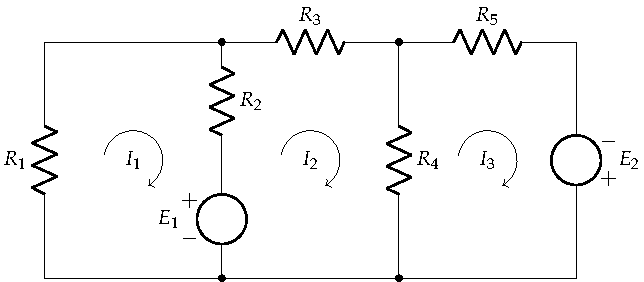
\includegraphics{figuras/BT1_02.pdf}
\end{center}

  

  \subsection*{Solución}
  Se plantea el sistema de ecuaciones en forma matricial, siendo de la forma $[R]\cdot[I]=[U]$. Cada $R_{i,i}$ de la matriz $[R]$ se corresponde con la suma de resistencias incluidas en la malla $i$; cada $\pm R_{ij}$ se corresponde con la suma de las resistencias incluidas en las ramas compartidas por las mallas $i$ y $j$, con signo positivo ($+$) si las corrientes van en el mismo sentido, y negativo ($-$) en caso contrario; y cada $\sum \epsilon_i$ es la suma algebraica de las fuerzas electromotrices de los generadores de la malla $i$, considerando un signo positivo ($+$) si contribuyen al giro de la corriente, y negativo ($-$) en caso contrario (es decir, si la corriente sale por el polo $+$ de la fuente, se considera positivo; si sale por el polo $-$, se considera negativo). Así:
  \begin{equation*}
    \begin{bmatrix}
      R_1+R_2 & -R_2 & 0 \\
      -R_2 & R_2+R_3+R_4 & -R_4 \\
      0 & -R_4 & R_4+R_5
    \end{bmatrix} \cdot
    \begin{bmatrix}
      I_1\\
      I_2\\
      I_3
    \end{bmatrix} = %
    \begin{bmatrix}
      -E_1 \\
      E_1\\
      E_2
    \end{bmatrix}
  \end{equation*}
  Reemplazando con los valores correspondientes, el sistema a resolver es:
  \begin{equation*}
    \begin{bmatrix}
      7 & -5 & 0 \\
      -5 & 19 & -4 \\
      0 & -4 & 6
    \end{bmatrix} \cdot
    \begin{bmatrix}
      I_1\\
      I_2\\
      I_3
    \end{bmatrix} = %
    \begin{bmatrix}
      -25 \\
      25\\
      50
    \end{bmatrix}
  \end{equation*}
  cuya solución es:
  \begin{align*}
    I_1&=\qty{-1.31}{\ampere}\\
    I_2&=\qty{3.17}{\ampere}\\
    I_3&=\qty{10.45}{\ampere}
  \end{align*}


%%%%%%%%%%%%%%%%%%%%%%%%%%%%%%%%%%%%%%%%%%%%%%%%%%%%%%%%%%%%%%%%%%%%%%%%%

  \section{Enunciado}
  Calcular el valor de $E$ que hace que $I_0=\qty{7.5}{\milli\ampere}$
  en el circuito de la figura.

\vspace{2mm}
Datos: $\; R_1 = \qty{8}{\ohm}$;\; $R_2 = \qty{7}{\ohm}$;\; $R_3 = \qty{4}{\ohm}$,\; $R_4 = \qty{6}{\ohm}$;\; $R_5 = \qty{6}{\ohm}$;\; $R_6 = \qty{12}{\ohm}$

  \begin{center}
    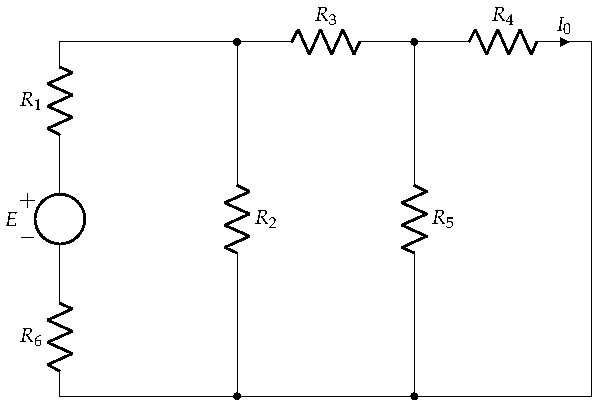
\includegraphics{figuras/BT1_03.pdf}
  \end{center}
   

\subsection*{Solución}
Siguiendo las mismas consideraciones del ejercicio anterior, se plantea el sistema de ecuaciones en forma matricial, suponiendo que
las tres corrientes de malla van en sentido horario:
\begin{equation*}
  \begin{bmatrix}
    R_1+R_2+R_6 & -R_2 & 0 \\
    -R_2 & R_2+R_3+R_5 & -R_5 \\
    0 & -R_5 & R_4+R_5
  \end{bmatrix} \cdot
  \begin{bmatrix}
    I_a\\
    I_b\\
    I_c
  \end{bmatrix} = %
  \begin{bmatrix}
    E \\
    0\\
    0
  \end{bmatrix}
\end{equation*}
Reemplazando con los valores correspondientes, el sistema a resolver es:
\begin{equation*}
  \begin{bmatrix}
    27 & -7 & 0 \\
    -7 & 17 & -6 \\
    0 & -6 & 12
  \end{bmatrix} \cdot
  \begin{bmatrix}
    I_a\\
    I_b\\
    I_c
  \end{bmatrix} = %
  \begin{bmatrix}
    E \\
    0\\
    0
  \end{bmatrix}
\end{equation*}
donde además se sabe el valor de $I_c=I_0=\qty{7.5}{\milli\ampere}$. Por
tanto, de la tercera ecuación se puede obtener el valor de $I_b$:
\begin{equation*}
  -6\,I_b+12\,I_c=-6\,I_b+12\cdot 7.5 = 0 \quad \Rightarrow \quad 6\,I_b=90 \quad \Rightarrow \quad I_b=\dfrac{90}{6}=\qty{15}{\milli\ampere}
\end{equation*}
Con $I_b$ calculado, se utiliza la segunda ecuación para determinar
$I_a$:
\begin{equation*}
  -7\,I_a+17\,I_b-6\,I_c=-7\,I_a+17\cdot 15-6\cdot 7.5 = 0\quad \Rightarrow \quad 7\,I_a=210\quad \Rightarrow \quad I_a=\dfrac{210}{7}=\qty{30}{\milli\ampere}
\end{equation*}
Determinada $I_a$, se emplea la primera ecuación para obtener el valor
de $E$:
\begin{equation*}
  27\,I_a-7\,I_b=27\cdot 30 - 7 \cdot 15 = E = {\qty{705}{\milli\volt}}
\end{equation*}


%%%%%%%%%%%%%%%%%%%%%%%%%%%%%%%%%%%%%%%%%%%%%%%%%%%%%%%%%%%%%%%%%%%%%%%%%

\section{Enunciado}
Calcular la intensidad $I$ en el circuito de la figura.

\vspace{2mm}
  Datos: $\; R_1 = \qty{27}{\ohm}$;\; $R_2 = \qty{47}{\ohm}$;\; $R_3 = \qty{27}{\ohm}$;\; $E_1 = \qty{460}{\volt}$;\; $E_2 = \qty{200}{\volt}$
  
\begin{center}
  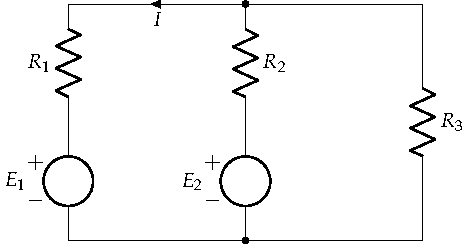
\includegraphics{figuras/BT1_04.pdf}
\end{center}


\subsection*{Solución}
Se suponen las mallas mostradas en la siguiente figura.

\begin{center}
  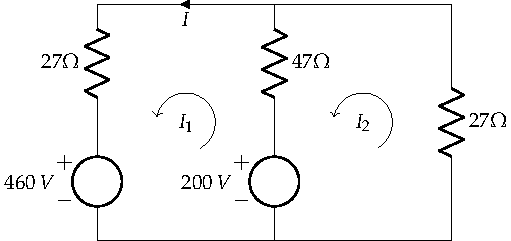
\includegraphics{figuras/BT1_04_mallas.pdf}
\end{center}

Se plantea el sistema de ecuaciones en forma matricial:
\begin{equation*}
  \begin{bmatrix}
    74 & -47  \\
    -47 & 74
  \end{bmatrix} \cdot
  \begin{bmatrix}
    I_1\\
    I_2
  \end{bmatrix} =
  \begin{bmatrix}
    -260 \\
    -200
  \end{bmatrix}
\end{equation*}
cuya solución es:
\begin{align*}
  I_1&=\qty{-8.77}{\ampere}\\
  I_2&=\qty{-8.27}{\ampere}
\end{align*}

%%%%%%%%%%%%%%%%%%%%%%%%%%%%%%%%%%%%%%%%%%%%%%%%%%%%%%%%%%%%%%%%%%
\section{Enunciado}
En el circuito de la figura obtener las intensidades de corriente
señaladas primero mediante un análisis por el método de las mallas y
posteriormente mediante un análisis por el método de los nudos.

\vspace{2mm}
Datos: $\; R_1 = \qty{2}{\ohm}$;\; $R_2 = \qty{1}{\ohm}$;\; $R_3 = \qty{4}{\ohm}$;\; $R_4 = \qty{5}{\ohm}$;\; $R_5 = \qty{3}{\ohm}$;\; $E_1 = \qty{10}{\volt}$;\; $E_2 = \qty{6}{\volt}$

\begin{center}
  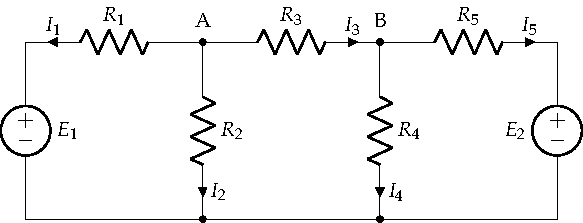
\includegraphics{figuras/BT1_08.pdf}
\end{center}
  

\subsection*{Solución}
Se aplica primero el método de las mallas, considerando las corrientes
de malla mostradas en la siguiente figura:
\begin{center}
  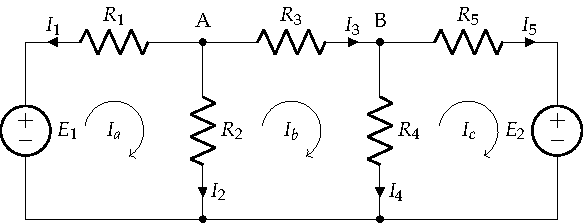
\includegraphics{figuras/BT1_08_mallas.pdf}
\end{center}

Se plantea el sistema de ecuaciones en forma matricial:
\begin{equation*}
  \begin{bmatrix}
    3 & -1 & 0 \\
    -1 & 10 & -5 \\
    0 & -5 & 8
  \end{bmatrix} \cdot
  \begin{bmatrix}
    I_a\\
    I_b\\
    I_c
  \end{bmatrix} = %
  \begin{bmatrix}
    10 \\
    0\\
    -6
  \end{bmatrix}
\end{equation*}
cuya solución es:
\begin{align*}
  I_a&=\qty{3.31}{\ampere}\\
  I_b&=\qty{-0.06}{\ampere}\\
  I_c&= \qty{-0.79}{\ampere}
\end{align*}
Se establecen las igualdades entre las diferentes corrientes de rama y
de malla, y se calculan sus valores:
\begin{align*}
  I_1&=-I_a=\qty{-3.31}{\ampere}\\
  I_2&=I_a-I_b=3.31-(-0.06)=\qty{3.37}{\ampere}\\
  I_3&=I_b=\qty{-0.06}{\ampere}\\
  I_4&=I_b-I_c=-0.06-(-0.79)=\qty{0.73}{\ampere}\\
  I_5&=I_c=\qty{-0.79}{\ampere}
\end{align*}
	
Para poder aplicar el método de los nudos, es necesario hacer, en
primer lugar, la transformación de las fuentes de tensión (y la
resistencia en serie) en fuentes de corriente (con una resistencia en
paralelo):
\begin{align*}
  I_{g,10V}&=\dfrac{\epsilon_{10V}}{R_{2\Omega}}=\dfrac{10}{2}=\qty{5}{\ampere}\\
  I_{g,6V}&=\dfrac{\epsilon_{6V}}{R_{3\Omega}}=\dfrac{6}{3}=\qty{2}{\ampere}
\end{align*}
quedando el circuito que se muestra a continuación.

\begin{center}
  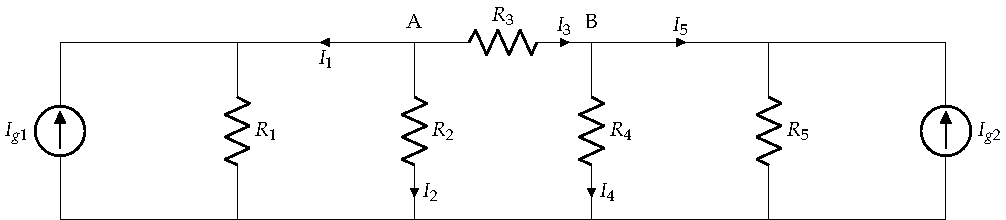
\includegraphics{figuras/BT1_08_nudos.pdf}
\end{center}

En este caso, se trabaja con las conductancias ($G=1/R$). Se
escribe el sistema de ecuaciones en modo matricial:
\begin{equation*}
  \begin{bmatrix}
    1.75 & - 0.25\\
    -0.25 & 0.783
  \end{bmatrix} \cdot%
  \begin{bmatrix}
    U_A\\
    U_B
  \end{bmatrix} = %
  \begin{bmatrix}
    5\\
    2
  \end{bmatrix}
\end{equation*}
cuya solución es:
\begin{align*}
  U_A&=\qty{3.38}{\volt}\\
  U_B&=\qty{3.63}{\volt}
\end{align*}
Con estos valores, se pueden determinar directamente las corrientes
$I_2$ e $I_4$, por simple aplicación de la ley de Ohm:
\begin{align*}
  I_2&=\dfrac{U_A}{R_{1\Omega}}=\dfrac{3.38}{1}=\qty{3.38}{\ampere}\\
  I_4&=\dfrac{U_B}{R_{5\Omega}}=\dfrac{3.63}{5}=\qty{0.73}{\ampere}
\end{align*}
Las corrientes que circulan por las resistencias en paralelo con las
fuentes de tensión se determinan de manera análoga:
\begin{align*}
  I_{2\Omega}&=\dfrac{U_A}{R_{2\Omega}}=\dfrac{3.38}{2}=\qty{1.69}{\ampere}\\
  I_{3\Omega}&=\dfrac{U_B}{R_{3\Omega}}=\dfrac{3.63}{3}=\qty{1.21}{\ampere}
\end{align*}
Por la 1LK, se determina el valor de $I_1$, $I_3$ e $I_5$:
\begin{align*}
  I_1&+5=I_{2\Omega} \quad \Rightarrow \quad I_1=I_{2\Omega}-5=1.69-5=\qty{-3.31}{\ampere}\\
  I_5&+2=I_{3\Omega} \quad \Rightarrow \quad I_5=I_{3\Omega}-2=1.21-2=\qty{-0.79}{\ampere}\\
  I_3&=I_4+I_5=0.73+(-0.79)=\qty{-0.06}{\ampere}
\end{align*}

Se observa que los resultados obtenidos con ambos métodos son
idénticos, con una pequeña diferencia en el segundo decimal de $I_2$, debida simplemente a aproximar a dos decimales en resultados parciales.

%%%%%%%%%%%%%%%%%%%%%%%%%%%%%%%%%%%%%%%%%%%%%%%%%%%%%%%%%%%%%%%%%%
\section{Enunciado}
Analizar el circuito de la figura mediante el método de las mallas,
obteniendo la corriente de cada una de las ramas. Con este resultado,
calcular la diferencia de potencial entre A y B, y realizar un balance
de potencias comparando la potencia de los elementos activos y la de
los elementos pasivos.

\vspace{2mm}
Datos:
$\; R_1 = R_2 = \qty{1}{\ohm};\; R_3 = \qty{2}{\ohm}; R_4 = \qty{3}{\ohm};\;
R_5=\qty{4}{\ohm};\; \epsilon_1=\qty{118}{\volt};\; \epsilon_2 =
\qty{236}{\volt};\; \epsilon_3 = \qty{118}{\volt}$

\begin{center}
  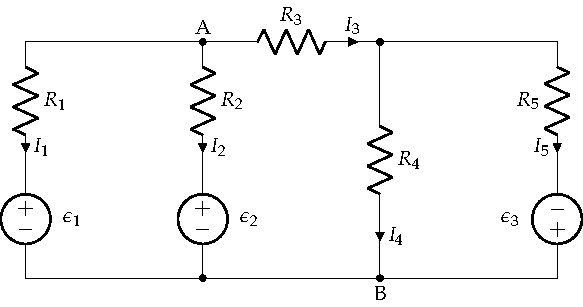
\includegraphics{figuras/mallas2.pdf}
\end{center}

\subsection*{Solución}
Se usan tres corrientes de malla con giro a derechas, de nombre (de
izquierda a derecha), $I_a$, $I_b$ e $I_c$. Escribiendo el sistema de
ecuaciones del método de las mallas en forma matricial:
\begin{equation*}
  \begin{bmatrix}
    2 & -1 & 0 \\
    -1 & 6 & -3 \\
    0 & -3 & 7
  \end{bmatrix}
  \cdot
  \begin{bmatrix}
    I_a\\
    I_b\\
    I_c
  \end{bmatrix}
  =
  \begin{bmatrix}
    -118\\
    236\\
    118
  \end{bmatrix}
\end{equation*}
cuya solución es:
\begin{align*}
  I_a &= \qty{-32}{\ampere}\\
  I_b &= \qty{54}{\ampere}\\
  I_c &= \qty{40}{\ampere}
\end{align*}

Estableciendo las relaciones entre las corrientes de rama y las
corrientes de malla, y sustituyendo, se llega a la conclusión de que:

\vspace{-4mm}
\begin{align*}
  I_1 &= -I_a=\qty{32}{\ampere}\\
  I_2 &= I_a - I_b=-32-54=\qty{-86}{\ampere}\\
  I_3 &= I_b=\qty{54}{\ampere}\\
  I_4 &= I_b - I_c=54-40=\qty{14}{\ampere}\\
  I_5 &= I_c=\qty{40}{\ampere}
\end{align*}

\emph{Se recomienda comprobar que estos resultados cumplen la 1LK en
  los nudos del circuito, para asegurarse de que la resolución es
  correcta.}

\vspace{4mm}
La diferencia de potencial entre A y B es:
\begin{equation*}
  U_{AB} = I_3 \cdot R_3 + I_4 \cdot R_4 = 54\cdot 2+14\cdot 3= \qty{150}{\volt}
\end{equation*}

La potencia entregada por los generadores del circuito es:

\vspace{-4mm}
\begin{align*}
  P_{\epsilon_1} &= \epsilon_1 \cdot (-I_1) = -\qty{3,776}{\kilo\watt}\\
  P_{\epsilon_2} &= \epsilon_2 \cdot (-I_2) = \qty{20,296}{\kilo\watt}\\
  P_{\epsilon_3} &= \epsilon_3 \cdot I_5 = \qty{4,72}{\kilo\watt}\\
  P_\epsilon &= P_{\epsilon_1} + P_{\epsilon_2} + P_{\epsilon_3} = \qty{21,24}{\kilo\watt}  
\end{align*}

Es importante recordar que el criterio de signos de un generador considera que la potencia entregada es positiva cuando la corriente sale del generador por su terminal positivo. Por tanto, $I_1$ e $I_2$ son empleadas con un signo negativo. En consecuencia, la potencia del generador $\epsilon_1$ es negativa, lo que quiere decir que este generador funciona como receptor (absorbe potencia). Ahora bien, dado que $I_2$ tiene valor negativo (es decir, circula en sentido contrario al indicado en la figura), la potencia del generador $\epsilon_2$ es positiva, de forma que este generador actúa como tal.

\vspace{3mm}
La potencia disipada por las resistencias es:

\vspace{-3mm}
\begin{align*}
  P_{R_1} &= I_1^2 \cdot R_1 = \qty{1,024}{\kilo\watt}\\
  P_{R_2} &= I_2^2 \cdot R_2 = \qty{7,396}{\kilo\watt}\\
  P_{R_3} &= I_3^2 \cdot R_3 = \qty{5,832}{\kilo\watt}\\
  P_{R_4} &= I_4^2 \cdot R_4 = \qty{588}{\watt}\\
  P_{R_5} &= I_5^2 \cdot R_5 = \qty{6,4}{\kilo\watt}\\
  P_R &= \sum_i P_{Ri} = \qty{21,24}{\kilo\watt}  
\end{align*}

Comprobamos que se cumple el balance de potencias.

%%%%%%%%%%%%%%%%%%%%%%%%%%%%%%%%%%%%%%%%%%%%%%%%%%%%%%%%%%%%%%%%%% 
\section{Enunciado}
En el circuito de la figura, se debe determinar:
\begin{itemize}
\item Todas las intensidades de rama señaladas.
\item Carga, polaridad y energía almacenada en los condensadores.
\item Balance de potencias.
\end{itemize}

  Datos: $ \; R_i = \qty[parse-numbers=false]{i}{\ohm}$; \; $C_i = \qty[parse-numbers=false]{i}{\micro\farad}$; \; $E_1 = \qty{8}{\volt}$; \; $E_2 = \qty{6}{\volt}$; \; $E_3 = \qty{4}{\volt}$

\begin{center}
  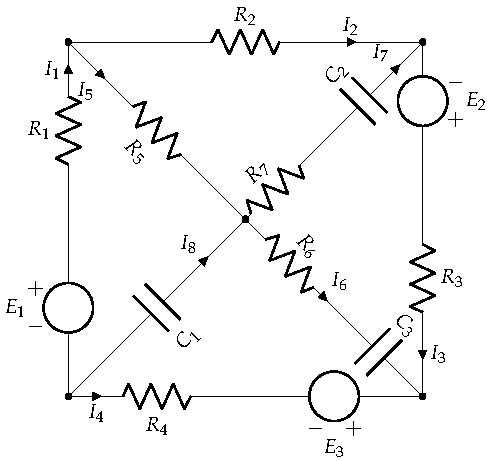
\includegraphics{figuras/BT1_09.pdf}
\end{center}


\subsection*{Solución}
Al tratarse de un circuito alimentado por corriente continua, los
condensadores se comportan como un circuito abierto, por lo que el
circuito a analizar es el mostrado en la figura.

\begin{center}
  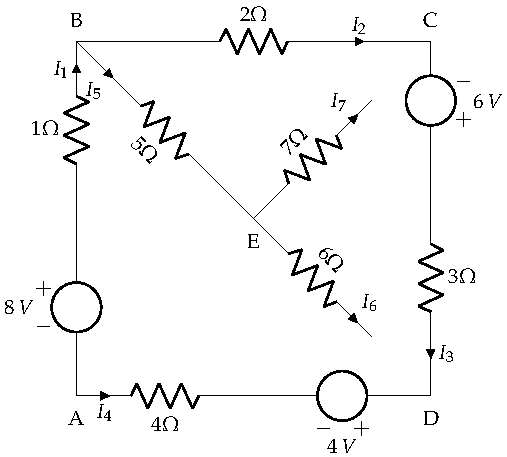
\includegraphics{figuras/BT1_09_sol.pdf}
\end{center}

Por simple observación, obtenemos:
\begin{equation*}
  I_5=I_6=I_7=\qty{0}{\ampere}
\end{equation*}
quedando una única malla por la que circula la misma corriente
$I_1=I_2=I_3=-I_4=I$. Por la 2LK, considerando que $I$ va en sentido
horario, se obtiene que:
\begin{equation*}
  -8+1\, I+2\,I-6+3\,I+4+4\,I=0 \quad \Rightarrow \quad {I = \dfrac{8+6-4}{1+2+3+4}=\qty{1}{\ampere}=I_1=I_2=I_3=-I_4}
\end{equation*}

Para determinar la carga de los condensadores hay que calcular las
tensiones en los diferentes nudos. Considerando $E$ como tierra:
\begin{align*}
  U_{AE}&=U_{A}-\cancelto{0}{U_{E}}=-8+1\,I_1+5\,I_5=-8+1\cdot 1 + 5\cdot 0=\qty{-7}{\volt}\\
  U_{CE}&=U_{C}-\cancelto{0}{U_{E}}=-2\,I_2+5\,I_5=-2\cdot 1+5\cdot 0 =\qty{-2}{\volt}\\
  U_{DE}&=U_{D}-\cancelto{0}{U_{E}}=4-4\, I_4-8+1\,I_1+5\,I_5=4-4\cdot (-1)-8+1\cdot 1 +5\cdot 0=\qty{1}{\volt}
\end{align*}
Con estas tensiones, se determina la carga de los condensadores:
\begin{align*}
  Q_{1\si{\micro\farad}} &= C_{1\si{\micro\farad}} \cdot U_{AE} = 1\cdot 10^{-6}\cdot (-7)=\qty{-7}{\micro\coulomb}\\
  Q_{2\si{\micro\farad}} &= C_{2\si{\micro\farad}} \cdot U_{CE} = 2\cdot 10^{-6}\cdot (-2)=\qty{-4}{\micro\coulomb}\\
  Q_{3\si{\micro\farad}} &= C_{3\si{\micro\farad}} \cdot U_{DE} = 3\cdot 10^{-6}\cdot 1=\qty{3}{\micro\coulomb}
\end{align*}
Aquellos condensadores en los que la carga es negativa, significa que
tienen la polaridad contraria a la considerada. La energía es:
\begin{align*}
  E_{1\si{\micro\farad}}&=\dfrac{1}{2}\,C_{1\si{\micro\farad}}\cdot U_{AE}^2 = \dfrac{1}{2}\cdot 1\cdot 10^{-6}\cdot (-7)^2 = \qty{24.5}{\micro\joule}\\
  E_{2\si{\micro\farad}}&=\dfrac{1}{2}\,C_{2\si{\micro\farad}}\cdot U_{CE}^2 = \dfrac{1}{2}\cdot 2\cdot 10^{-6}\cdot (-2)^2 = \qty{4}{\micro\joule}\\
  E_{3\si{\micro\farad}}&=\dfrac{1}{2}\,C_{3\si{\micro\farad}}\cdot U_{DE}^2 = \dfrac{1}{2}\cdot 3\cdot 10^{-6}\cdot 1^2 = \qty{1.5}{\micro\joule}
\end{align*}

Se calculan las potencias de los elementos activos y las potencias consumidas por las resistencias:
\begin{itemize}
\item Potencias de los elementos activos:
    \begin{align*}
      P_{E1} &= E_1 \cdot I_1 = \qty{8}{\watt}\\
      P_{E2} &= E_2 \cdot I_3 = \qty{6}{\watt}\\
      P_{E3} &= E_3 \cdot I_4 = -\qty{4}{\watt}
    \end{align*}
\item Potencias de las resistencias:
    \begin{align*}
      P_{R,1}&= R_1 \cdot I_1^2=1\cdot 1^2 = \qty{1}{\watt}\\
      P_{R,2}&= R_2 \cdot I_2^2=2\cdot 1^2 = \qty{2}{\watt}\\
      P_{R,3}&= R_3 \cdot I_3^2=3\cdot 1^2 = \qty{3}{\watt}\\
      P_{R,4}&= R_4 \cdot I_4^2=4\cdot (-1)^2 = \qty{4}{\watt}
    \end{align*}
\end{itemize}
Donde se cumple que la potencia total aportada por los generadores es igual a la potencia consumida por las resistencias.

%%%%%%%%%%%%%%%%%%%%%%%%%%%%%%%%%%%%%%%%%%%%%%%%%%%%%%%%%%%%%%%%%% 

\section{Enunciado}
Aplicar el método de los nudos en el circuito de la figura para
determinar:
\begin{itemize}
\item Los potenciales de los nudos A, B, C y D.
\item Las intensidades de corriente señaladas.
\item Carga, polaridad y energía almacenada en los condensadores,
  supuestos sin carga inicial.
\end{itemize}
Datos:
$ \; R_i = \qty[parse-numbers=false]{i}{\ohm}$; \; $C_i = \qty[parse-numbers=false]{i}{\micro\farad}$; \; $\epsilon_1 = \qty{6}{\volt}$; \; $\epsilon_2 =
\qty{18}{\volt}$; \; $\epsilon_3 = \qty{6}{\volt}$

\begin{center}
  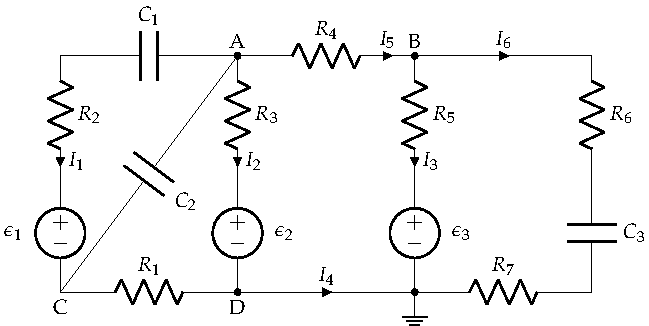
\includegraphics[]{figuras/nudos_condensadores.pdf}
\end{center}

\subsection*{Solución}

Sustituimos los condensadores por circuitos abiertos. En consecuencia, por las ramas correspondientes no puede circular corriente:

\vspace{2mm}
\begin{minipage}{0.65\linewidth}
  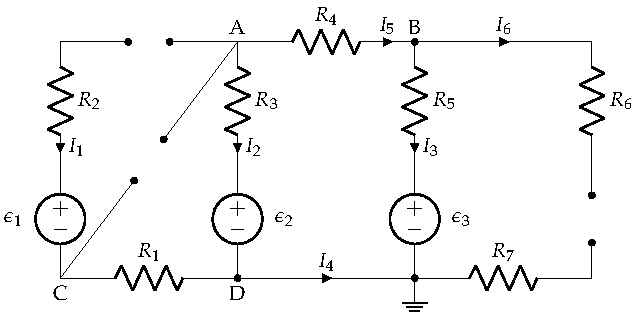
\includegraphics[scale=1]{figuras/nudos_condensadores2.pdf}
\end{minipage}
\begin{minipage}{0.25\linewidth}
    \begin{align*}
      I_1 &= \qty{0}{\ampere}\\
      I_6 &= \qty{0}{\ampere}
    \end{align*}    
\end{minipage}

\vspace{6mm}
Luego el circuito equivalente es:

\vspace{2mm}
\begin{minipage}{0.32\linewidth}
    \begin{center}
        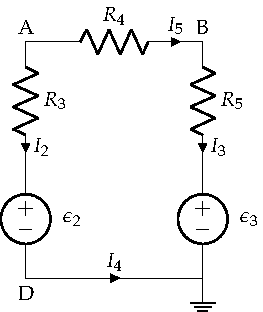
\includegraphics[scale=1]{figuras/nudos_condensadores3.pdf}
    \end{center}
\end{minipage}
\begin{minipage}[c]{0.08\linewidth}
    \begin{center}
    $\LARGE \xrightarrow{\hspace*{0.5cm}}$ % https://latex.org/forum/viewtopic.php?t=3894
    \end{center}
\end{minipage}    
\begin{minipage}{0.6\linewidth}
    \begin{center}
        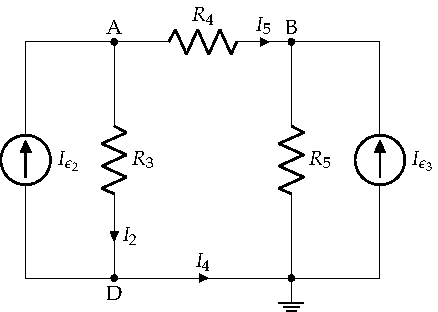
\includegraphics[scale=1]{figuras/nudos_condensadores4.pdf}
    \end{center}
\end{minipage}

\vspace{4mm}
Donde hemos transformado las fuentes de tensión en fuentes de corriente, para poder aplicar el método de los nudos.

\vspace{3mm}
Formulando la ecuación general del método de los nudos:

\begin{equation*}
  \begin{bmatrix}
    G_3 + G_4 & -G_4\\
    -G_4 & G_5 + G_4\\
  \end{bmatrix} \cdot %
  \begin{bmatrix}
    V_A\\
    V_B
  \end{bmatrix} = %
  \begin{bmatrix}
    \epsilon_2/R_3\\
    \epsilon_3/R_5
  \end{bmatrix}
\end{equation*}

\vspace{4mm}
Sustituyendo valores y resolviendo:

\vspace{-6mm}
\begin{align*}
  V_A &= \qty{15}{\volt}\\
  V_B &= \qty{11}{\volt}
\end{align*}

Además, $V_D = \qty{0}{\volt}$ , dado que está conectado a tierra. Por otra parte, la caída de tensión en la resistencia $R_1$ es de $\qty{0}{\volt}$, dado que $I_1 = \qty{0}{\ampere}$, luego $V_C = V_D = \qty{0}{\volt}$.

\vspace{4mm}

Con estos resultados podemos obtener los valores de las corrientes de rama. Volvemos al circuito original para plantear las ecuaciones de rama:

\vspace{-4mm}
\begin{align*}
  V_A &= I_2 \cdot R_3 + \epsilon_2\\
  V_B &= I_3 \cdot R_5 + \epsilon_3
\end{align*}

De estas ecuaciones despejamos $I_2$ e $I_3$. Además, teniendo en cuenta que $I_1 = I_6 = 0$, tenemos:

\vspace{-3mm}
\begin{align*}
  I_5 &= I_3\\
  I_4 &= I_2\\
  I_2 &= -I_3
\end{align*}

\vspace{-3mm}
En definitiva:

\vspace{-3mm}
\begin{align*}
  I_1 &= \qty{0}{\ampere}\\
  I_2 &= \qty{-1}{\ampere}\\
  I_3 &= \qty{1}{\ampere}\\
  I_4 &= \qty{-1}{\ampere}\\
  I_5 &= \qty{1}{\ampere}\\
  I_6 &= \qty{0}{\ampere}
\end{align*}

Finalmente, calculamos las diferencias de potencial en los
condensadores. En $C_1$ asignamos la polaridad positiva en A, y
tenemos:

\vspace{-2mm}
\begin{equation*}
  U_{AC} = U_{C_1} + \epsilon_1 \quad \rightarrow \quad U_{C_1} = \qty{9}{\volt}
\end{equation*}

\vspace{2mm}
Para $C_2$ y $C_3$, el cálculo es directo. Asignando la polaridad positiva en A y B, respectivamente:

\vspace{-4mm}
\begin{align*}
  U_{C_2} &=  U_{AC} = \qty{15}{\volt}\\
  U_{C_3} &=  U_{BD} = \qty{11}{\volt}
\end{align*}

\vspace{2mm}
En consecuencia, las cargas almacenadas en cada condensador son:

\vspace{-4mm}
\begin{align*}
  q_1 &= C_1 \cdot U_{C_1} = \qty{9}{\micro\coulomb}\\
  q_2 &= C_2 \cdot U_{C_2} = \qty{30}{\micro\coulomb}\\
  q_3 &= C_3 \cdot U_{C_3} = \qty{33}{\micro\coulomb}
\end{align*}

Y las energías almacenadas:

\vspace{-4mm}
\begin{align*}
  E_{C_1} &= \frac{1}{2} \cdot C_1 \cdot (U_{C_1})^2 = \qty{40.5}{\micro\joule}\\
  E_{C_2} &= \frac{1}{2} \cdot C_2 \cdot (U_{C_2})^2 = \qty{225}{\micro\joule}\\
  E_{C_3} &= \frac{1}{2} \cdot C_3 \cdot (U_{C_3})^2 = \qty{181.5}{\micro\joule}
\end{align*}

%%%%%%%%%%%%%%%%%%%%%%%%%%%%%%%%%%%%%%%%%%%%%%%%%%%%%%%%%%%%%%%%%% 

\section{Enunciado}

En el circuito de la figura, donde se sabe que la carga inicial de los
condensadores era de $\qty{10}{\micro\coulomb}$ para $C_1$ y de
$\qty{20}{\micro\coulomb}$ para $C_2$, con las polaridades indicadas,
se pide determinar:
\begin{itemize}
\item Intensidades de corriente señaladas.
\item Potenciales en los puntos A, B, C, D, E y F.
\end{itemize}

Datos:
$\; \epsilon_1=\qty{90}{\volt};\; \epsilon_2=\qty{60}{\volt};\;
\epsilon_3=\qty{30}{\volt};\; R_{1}= R_2 = R_3 =
\qty{10}{\ohm};\; R_{4}= R_5 = \qty{30}{\ohm};\; C_{1}=
\qty{10}{\micro\farad};\; C_{2}= \qty{20}{\micro\farad};\; L_1 =
\qty{1}{\micro\henry}$

\begin{center}
  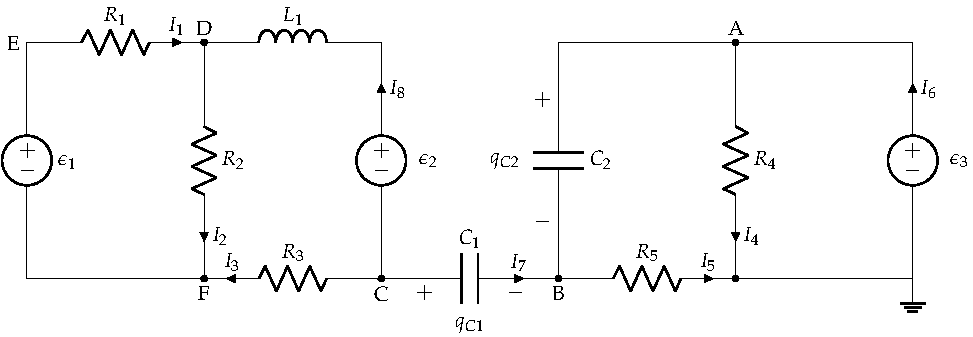
\includegraphics[scale = 0.9]{figuras/mallas_carga_inicial.pdf}
\end{center}


\subsection*{Solución}

Sustituimos los condensadores por circuitos abiertos, lo que implica que por las ramas correspondientes no puede circular corriente:

\vspace{-4mm}
\begin{align*}
  I_5 &= \qty{0}{\ampere}\\
  I_7 &= \qty{0}{\ampere}
\end{align*}

\begin{center}
  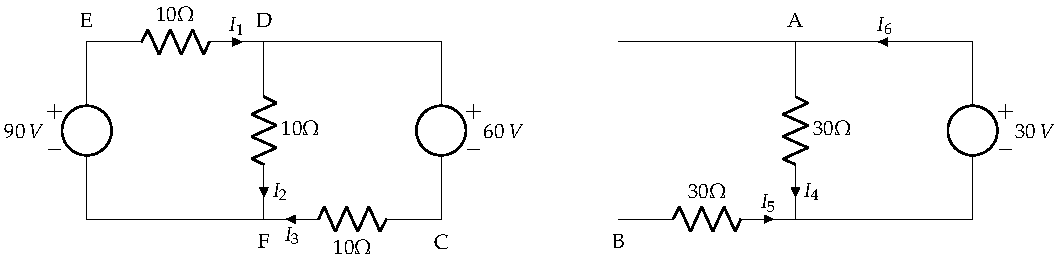
\includegraphics[width=\linewidth]{figuras/BT1_10_mod.pdf}
\end{center}

En consecuencia:

\vspace{-4mm}
\begin{align*}
  I_3 &= -I_8\\
  I_4 &= I_6
\end{align*}

\vspace{2mm}
Además, la bobina $L_1$ se sustituye por un cortocircuito.

\vspace{3mm}
Dado que el circuito original está ``partido'' en dos porciones inconexas, podemos analizar de manera independiente cada una de las dos porciones. Si aplicáramos la ecuación general de mallas al circuito en su conjunto, obtendríamos una matriz con ceros en los elementos comunes entre la malla 3 (malla en la que se incluye el generador 3), y las mallas 1 y 2, por lo que el sistema de ecuaciones $3\times 3$ sería separable en dos partes (de dimensiones $2\times 2$ y $1\times 1$).

\vspace{5mm}
Por lo tanto, en el circuito de la izquierda se tienen dos mallas, considerando las corrientes de malla mostradas en la siguiente figura:

\begin{center}
  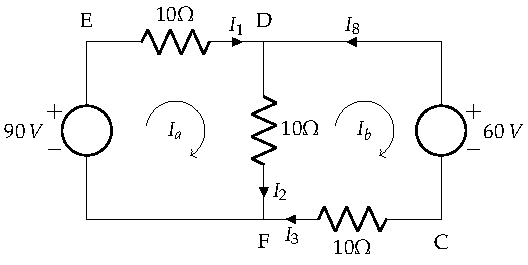
\includegraphics{figuras/BT1_10_izq_mallas.pdf}
\end{center}


\begin{equation*}
  \begin{bmatrix}
    R_1 + R_2 & -R_2\\
    -R_2 & R_2 + R_3\\
  \end{bmatrix} \cdot %
  \begin{bmatrix}
    I_a\\
    I_b
  \end{bmatrix} = %
  \begin{bmatrix}
    \epsilon_1\\
    -\epsilon_2
  \end{bmatrix}
\end{equation*}

\vspace{2mm}
La solución de este sistema es:

\vspace{-4mm}
\begin{align*}
  I_a &= \qty{4}{\ampere}\\
  I_b &= \qty{-1}{\ampere}
\end{align*}

\vspace{-4mm}
siendo,

\vspace{-4mm}
\begin{align*}
  I_1 &= I_a\\
  I_2 &= I_a - I_b\\
  I_3 &= I_b\\
  I_8 &= -I_b
\end{align*}

En el circuito de la derecha tenemos una única malla:

\begin{equation*}
  \epsilon_3 = I_4 \cdot R_4 \rightarrow I_4 = \qty{1}{\ampere}
\end{equation*}

Por tanto:
\begin{align*}
  I_1 &= \qty{4}{\ampere}\\
  I_2 &= \qty{5}{\ampere}\\
  I_3 &= \qty{-1}{\ampere}\\
  I_4 &= \qty{1}{\ampere}\\
  I_5 &= \qty{0}{\ampere}\\
  I_6 &= \qty{1}{\ampere}\\
  I_7 &= \qty{0}{\ampere}\\
  I_8 &= \qty{1}{\ampere}\\
\end{align*}

Para calcular los potenciales en los puntos A y B:

\vspace{-3mm}
\begin{align*}
  V_A &= \epsilon_3 = \qty{30}{\volt}\\
  V_B &= R_5 \cdot I_5 = \qty{0}{\volt}
\end{align*}

Para calcular el potencial en el punto C, debemos tener en cuenta que el condensador $C_1$ conserva su carga inicial porque el circuito no está cerrado en la parte superior. Por tanto:

\begin{equation*}
  U_{CB} = U_{C_1} = \frac{q_{C_1,0}}{C_1} = \qty{1}{\volt}
\end{equation*}
(para comprobar que nunca circula corriente por un elemento que esté conectado como $C_1$, se puede aplicar 1LK en los nudos D, F, y C, y sumando las 3 ecs. se obtiene que $I_7 = 0$)

\vspace{3mm}
Luego:

\vspace{-3mm}
\begin{equation*}
  U_C = U_{CB} + U_B = \qty{1}{\volt}
\end{equation*}

\vspace{2mm}
A partir de este resultado, podemos calcular el resto de potenciales:

\vspace{-3mm}
\begin{align*}
  U_D &= U_{DC} + U_C = \epsilon_2 + U_C = \qty{61}{\volt}\\
  U_E &= U_{ED} + U_D = I_1 \cdot R_1 + U_D = \qty{101}{\volt}\\
  U_F &= U_{FC} + U_C = -I_3 \cdot R_3 + U_C = \qty{11}{\volt}
\end{align*}

%%%%%%%%%%%%%%%%%%%%%%%%%%%%%%%%%%%%%%%%%%%%%%%%%%%%%%%%%%%%%%%%%% 
\section{Enunciado}
En el circuito de la figura, los condensadores se conectaron sin
carga. Mediante el método de las mallas, se pide determinar:
\begin{itemize}
\item Intensidades de corriente señaladas.
\item Potenciales en los puntos A, B, C y D.
\item Polaridades, cargas, y energías de los condensadores.
\item Balance de potencias.
\end{itemize}
\begin{minipage}[c]{0.2\linewidth}
  \begin{align*}
    \epsilon_{1}&=\qty{118}{\volt}\\
    \epsilon_{2}&=\qty{236}{\volt}\\
    \epsilon_{3}&=\qty{118}{\volt}\\
    R_{1}&= \qty{4}{\ohm}\\
    R_{2}&=R_{3}=\qty{1}{\ohm}\\
    R_{4}&= \qty{3}{\ohm}\\
    R_{5}&= \qty{2}{\ohm}\\
    C_{1}&=C_{2}=C_{3}=\qty{2}{\micro\farad}\\
    L_1 &= L_2 = L_3 = \qty{1}{\milli\henry}\\
  \end{align*}
\end{minipage}
\begin{minipage}[c]{0.8\linewidth}
  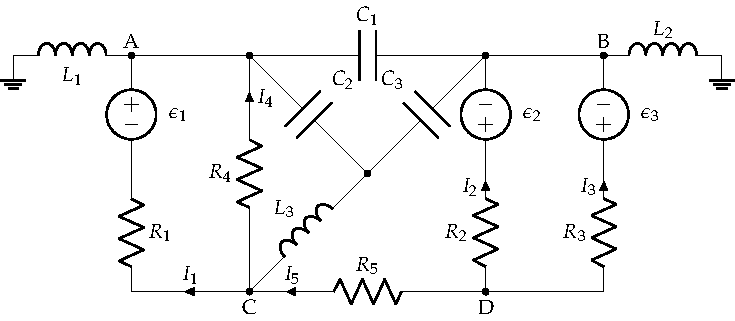
\includegraphics{figuras/mallas_condensadores.pdf}
\end{minipage}

\subsection*{Solución}
Se sustituyen los condensadores y las bobinas por sus equivalentes en un circuito de corriente continua (circuito abierto y cortocircuito, respectivamente). Por otro lado, dado que hay dos tomas de tierra en el esquema, esto no implica que haya dos referencias de potencial distintas: simplemente indica que esos dos puntos están cortocircuitados. En el circuito resultante, se definen tres corrientes de malla, como se muestra en el circuito de la figura:

\begin{center}            
    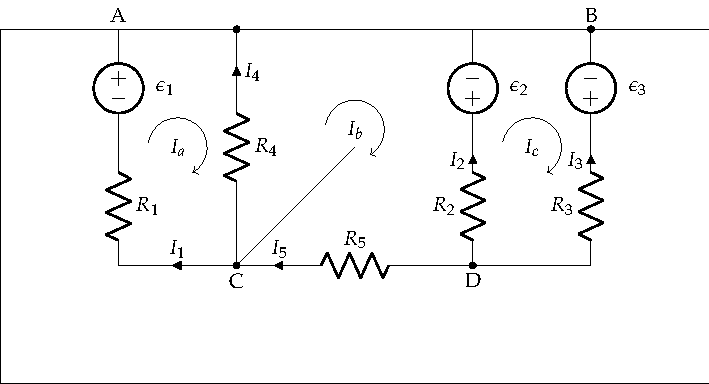
\includegraphics{figuras/mallas_condensadores_sol.pdf}
\end{center}
(la malla $b$ puede definirse de esta forma porque los puntos A y B están cortocircuitados)

\vspace{4mm}
Usamos la ecuación general del método de mallas:    
\begin{equation*}
    \begin{bmatrix}
        R_1 + R_4 & -R_4 & 0\\
        -R_4 & R_4 + R_5 + R_2 & -R_{2}\\
        0 & -R_2 & R_2 + R_3
    \end{bmatrix} \cdot %
    \begin{bmatrix}
        I_{a}\\
        I_{b}\\
        I_{c}
    \end{bmatrix} = %
    \begin{bmatrix}
        \epsilon_1\\
        \epsilon_2\\
        \epsilon_3 - \epsilon_2
    \end{bmatrix}
\end{equation*} 

\begin{equation*}
    \begin{bmatrix}
        7 & -3 & 0\\
        -3 & 6 & -1\\
        0 & -1 & 2
    \end{bmatrix} \cdot %
    \begin{bmatrix}
        I_{a}\\
        I_{b}\\
        I_{c}
    \end{bmatrix} = %
    \begin{bmatrix}
        118\\
        236\\
        -118
    \end{bmatrix}
\end{equation*}  

Cuya solución es:

\vspace{-6mm}
\begin{eqnarray*}
I_a & = & \qty{40}{\ampere}\\
I_b & = & \qty{54}{\ampere}\\
I_c & = & -\qty{32}{\ampere}
\end{eqnarray*}

Por tanto, las corrientes indicadas en el circuito son:

\vspace{-4mm}
\begin{eqnarray*}
I_1 & = & \qty{40}{\ampere}\\
I_2 & = & \qty{-86}{\ampere}\\
I_3 & = &  \qty{32}{\ampere}\\
I_4 & = &  \qty{14}{\ampere}\\
I_5 & = &  \qty{54}{\ampere}
\end{eqnarray*}

Los potenciales en los puntos indicados son:

\vspace{-4mm}
\begin{align*}
V_A &= \qty{0}{\volt}\\
V_B &= \qty{0}{\volt}\\
V_C &= I_4 \cdot R_4 = \qty{42}{\volt}\\
V_D &= I_5 \cdot R_5 + V_C = \qty{150}{\volt}\\
\end{align*}

\vspace{-2mm}
Por tanto, las polaridades de los condensadores y sus valores de tensión son los siguientes:

\vspace{-3mm}
\begin{eqnarray*}
    U_{C_1} = U_{BA} & = & \qty{0}{\volt}\\
    q_1 = C_1 \cdot U_{C_1} & = & \boxed{\qty{0}{\coulomb}}\\
    E_{C_1} = \frac{1}{2} C_1 \cdot (U_{C_1})^2 & = & \boxed{\qty{0}{\joule}}
\end{eqnarray*}

\vspace{-4mm}
\begin{eqnarray*}
    U_{C_2} = U_{CA} & = & \qty{42}{\volt}\\
    q_2 = C_2 \cdot U_{C_2} & = & \boxed{\qty{84}{\micro\coulomb}}\\
    E_{C_2} = \frac{1}{2} C_2 \cdot (U_{C_2})^2 & = & \boxed{\qty{1.76}{\milli\joule}}
\end{eqnarray*}

\vspace{-4mm}
\begin{eqnarray*}
    U_{C_3} = U_{CB} & = & \qty{42}{\volt}\\
    q_3 = C_3 \cdot U_{C_3} & = & \boxed{\qty{84}{\micro\coulomb}}\\
    E_{C_3} = \frac{1}{2} C_3 \cdot (U_{C_3})^2 & = & \boxed{\qty{1.76}{\milli\joule}}
\end{eqnarray*}

\vspace{5mm}
Finalmente, podemos formular el balance de potencias como potencia entregada por los elementos activos frente a potencia consumida por los elementos pasivos:

\vspace{1mm}
\begin{itemize}
    \item La potencia total entregada por los elementos activos es $\qty{21240}{\watt}$:
\end{itemize}

\vspace{-7mm}
\begin{eqnarray*}
P_{\epsilon_1} = \epsilon_1 \cdot I_1 & = & \qty{4720}{\watt}\\
P_{\epsilon_2} = \epsilon_2 \cdot (-I_2) & = & \qty{20296}{\watt}\\
P_{\epsilon_3} = \epsilon_3 \cdot (-I_3) & = & \qty{-3776}{\watt}
\end{eqnarray*}

\vspace{0.5mm}
\begin{itemize}
    \item La potencia total consumida por los elementos pasivos también es $\qty{21240}{\watt}$:
\end{itemize}

\vspace{-6mm}
\begin{eqnarray*}
P_{R_1} = R_1 \cdot (I_1)^2 & = & \qty{6400}{\watt}\\
P_{R_2} = R_2 \cdot (I_2)^2 & = & \qty{7396}{\watt}\\
P_{R_3} = R_3 \cdot (I_3)^2 & = & \qty{1024}{\watt}\\
P_{R_4} = R_4 \cdot (I_4)^2 & = & \qty{588}{\watt}\\
P_{R_5} = R_5 \cdot (I_5)^2 & = & \qty{5832}{\watt}
\end{eqnarray*}

%%%%%%%%%%%%%%%%%%%%%%%%%%%%%%%%%%%%%%%%%%%%%%%%%%%%%%%%%%%%%%%%%% 
\section{Enunciado}
En el circuito de la figura, determinar:
\begin{itemize}
\item Las ecuaciones para el cálculo de las intensidades.
\item Todas las intensidades indicadas.
\item Potenciales en todos los nudos.
\item Carga y energía almacenada en los condensadores.
\end{itemize}

\vspace{2mm}
  Datos: $R_1 = \qty{2}{\ohm}$; $R_2 = \qty{4}{\ohm}$; $R_3 = \qty{2}{\ohm}$; $R_4 = \qty{1}{\ohm}$; $R_5 = \qty{2}{\ohm}$; $R_6 = \qty{1}{\ohm}$; $E_1 = \qty{8}{\volt}$; $E_2 = \qty{8}{\volt}$; $C_i = \qty[parse-numbers=false]{i}{\micro\farad}$

\begin{center}
  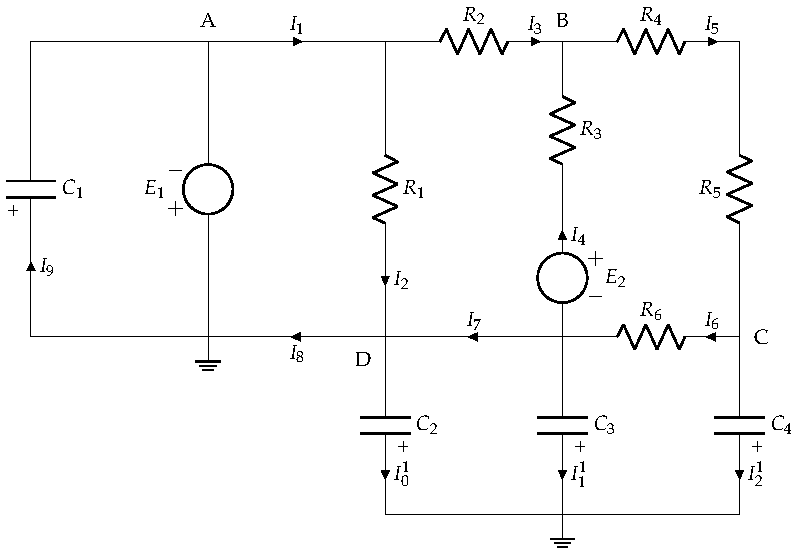
\includegraphics{figuras/BT1_11.pdf}
\end{center}

\subsection*{Solución}
Al tratarse de alimentación en CC, se sustituyen los condensadores por
circuitos abiertos, quedando el circuito de la figura:
\begin{center}
  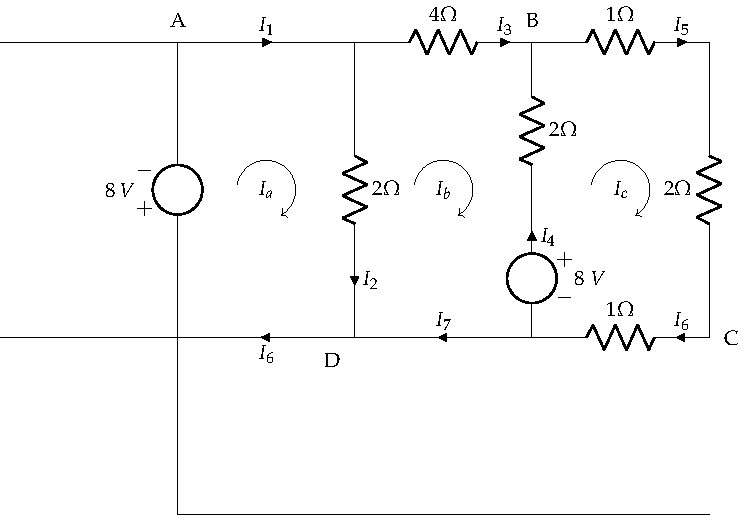
\includegraphics{figuras/BT1_11_mod.pdf}
\end{center}

Aplicando el método de mallas, con las corrientes indicadas, se
plantea el sistema de ecuaciones en forma matricial:
\begin{equation*}
  \begin{bmatrix}
    2 & -2 & 0 \\
    -2 & 8 & -2 \\
    0 & -2 & 6
  \end{bmatrix} \cdot
  \begin{bmatrix}
    I_a\\
    I_b\\
    I_c
  \end{bmatrix} = %
  \begin{bmatrix}
    -8 \\
    -8\\
    8
  \end{bmatrix}
\end{equation*}

\vspace{2mm}
Las ecuaciones completas para calcular las intensidades son:
\begin{align*}
  2\,I_a&-2\,I_b = -8\\
  -2\,I_a&+8\,I_b-2\,I_c = -8\\
  -2\,I_b&+ 6\,I_c = 8
\end{align*}
Cuya solución es:
\begin{align*}
  I_a&=\qty{-6.5}{\ampere}\\
  I_b&=\qty{-2.5}{\ampere}\\
  I_c&=\qty{0.5}{\ampere}\\
\end{align*}

Estableciendo las relaciones entre las corrientes de malla y las de rama del circuito:
\begin{align*}
  I_1&=I_8=I_a= \boxed{\qty{-6.5}{\ampere}}\\
  I_2&=I_a-I_b=-6.5-(-2.5)= \boxed{\qty{-4}{\ampere}}\\
  I_3&=I_7=I_b= \boxed{\qty{-2.5}{\ampere}}\\
  I_4&=I_c-I_b=0.5-(-2.5)= \boxed{\qty{3}{\ampere}}\\
  I_5&=I_6=I_c= \boxed{\qty{0.5}{\ampere}}\\
\end{align*}

\vspace{-2mm}
Una forma alternativa de resolver el circuito consiste en reparar en que $E_1$ es generador dominante, por lo que puede determinarse directamente el valor de $I_2 = - E_1 / R_1 = -4\si{\ampere}$. Esto permite usar únicamente 2 mallas, lo que reduce el sistema de ecuaciones a $2\times 2$: 

\vspace{4mm}
\begin{minipage}{0.6\linewidth}
    \begin{center}
    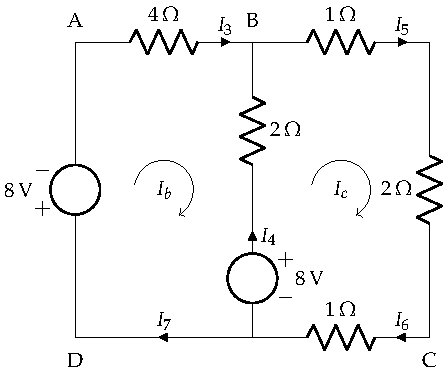
\includegraphics[scale=1]{figuras/BT1_11_mod2.pdf}
    \end{center}
\end{minipage}
\hfill
\begin{minipage}{0.3\linewidth}
    \begin{equation*}
      \begin{bmatrix}
        6 & -2  \\
        -2 & 6
      \end{bmatrix} \cdot
      \begin{bmatrix}
        I_b\\
        I_c
      \end{bmatrix} = %
      \begin{bmatrix}
        -16\\
        8
      \end{bmatrix}
    \end{equation*}

    \vspace{6mm}
    
    Cuya solución es la misma que 
    
    la obtenida anteriormente.
\end{minipage}

\vspace{4mm}
Conociendo las corrientes y teniendo el nudo de tierra como referencia, se calculan los potenciales:
\begin{align*}
  U_A&=-U_{8\si{\volt}}= \boxed{\qty{-8}{\volt}}\\
  U_B&=-U_{R2\Omega}+U_{8\si{\volt}}=-2\cdot 3+8= \boxed{\qty{2}{\volt}}\\
  U_C&=U_{R1\Omega}=1\cdot 0.5= \boxed{\qty{0.5}{\volt}}\\
  U_D&= \boxed{\qty{0}{\volt}}
\end{align*}

\vspace{4mm}
Con los potenciales, se determina la carga de los condensadores:
\begin{align*}
  Q_{1\si{\micro\farad}}&=C_{1\si{\micro\farad}}\, (-U_{A}) = 1\cdot 10^{-6}\cdot (-(-8))= \boxed{\qty{8}{\micro\coulomb}}\\
  Q_{2\si{\micro\farad}}&=C_{2\si{\micro\farad}} \cdot \qty{0}{\volt} = \boxed{\qty{0}{\micro\coulomb}}\\
  Q_{3\si{\micro\farad}}&=C_{3\si{\micro\farad}} \cdot \qty{0}{\volt} = \boxed{\qty{0}{\micro\coulomb}}\\
  Q_{4\si{\micro\farad}}&=C_{4\si{\micro\farad}}\, (-U_C) = 4\cdot 10^{-6}\cdot (-0.5)= \boxed{\qty{-2}{\micro\coulomb}}
\end{align*}

\vspace{4mm}
Aquellos condensadores en los que la carga es negativa, significa que tienen polaridad contraria a la considerada. La energía almacenada en cada uno de ellos es:

\begin{align*}
  E_{1\si{\micro\farad}}&=\dfrac{1}{2}\,C_{1\si{\micro\farad}}\cdot (-U_{A})^2 = \dfrac{1}{2}\cdot 1\cdot 10^{-6}\cdot (-(-8))^2= \boxed{\qty{32}{\micro\joule}}\\
  E_{2\si{\micro\farad}}&= \boxed{\qty{0}{\micro\joule}}\\
  E_{3\si{\micro\farad}}&= \boxed{\qty{0}{\micro\joule}}\\
  E_{4\si{\micro\farad}}&=\dfrac{1}{2}\,C_{4\si{\micro\farad}}\cdot (-U_{C})^2 = \dfrac{1}{2}\cdot 4\cdot 10^{-6}\cdot (-0.5)^2= \boxed{\qty{0.5}{\micro\joule}}
\end{align*}

%%%%%%%%%%%%%%%%%%%%%%%%%%%%%%%%%%%%%%%%%%%%%%%%%%%%%%%%%%%%%%%%%%
\section{Enunciado}
En el circuito de la figura se debe determinar:
\begin{itemize}
\item Las corrientes señaladas.
\item El balance de potencias, diferenciando entre elementos activos y
  elementos pasivos.
\item Los potenciales en los puntos A, B y C.
\item La carga y polaridad en los condensadores, supuestos sin carga
  inicial.
\end{itemize}
\begin{minipage}[c]{0.25\linewidth}
  \begin{align*}
    \epsilon_1&=\qty{1}{\volt}\\
    \epsilon_2&=\qty{7}{\volt}\\
    R_i &= \qty{1}{\ohm}\\
    C_i &= \qty[parse-numbers=false]{i}{\micro\farad}
  \end{align*}
\end{minipage}
\begin{minipage}[c]{0.75\linewidth}
  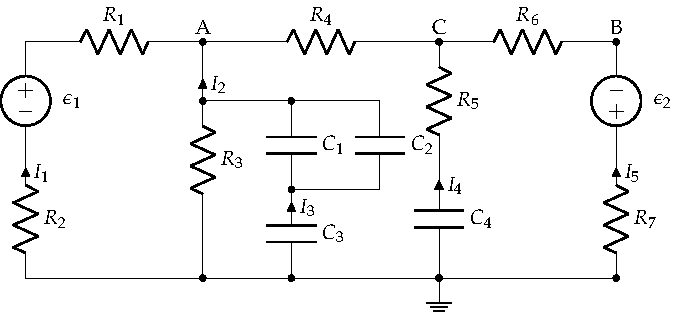
\includegraphics{figuras/mallas_agrupacion_condensadores.pdf}
\end{minipage}

\subsection*{Solución}
Sustituimos los condensadores por circuitos abiertos. En consecuencia, por las ramas correspondientes no puede circular corriente:

\vspace{-4mm}
\begin{align*}
  I_3 &= \boxed{\qty{0}{\ampere}}\\
  I_4 &= \boxed{\qty{0}{\ampere}}
\end{align*}

Tenemos dos mallas, y definimos dos corrientes de malla dextrógiras (sentido horario):

\begin{equation*}
  \begin{bmatrix}
    R_1 + R_2 + R_3 & -R_3\\
    -R_3 & R_3 + R_4 + R_6 + R_7\\
  \end{bmatrix} \cdot %
  \begin{bmatrix}
    I_a\\
    I_b
  \end{bmatrix} = %
  \begin{bmatrix}
    \epsilon_1\\
    \epsilon_2
  \end{bmatrix}
\end{equation*}

\vspace{3mm}
La solución de este sistema es:

\vspace{-5mm}
\begin{align*}
  I_a &= \qty{1}{\ampere}\\
  I_b &= \qty{2}{\ampere}
\end{align*}

\vspace{-1mm}
siendo,

\vspace{-5mm}
\begin{align*}
  I_1 &= I_a = \boxed{\qty{1}{\ampere}}\\
  I_2 &= I_b - I_a = \boxed{\qty{1}{\ampere}}\\
  I_5 &= -I_b = \boxed{\qty{-2}{\ampere}}
\end{align*}

\vspace{2mm}
La potencia de los dos elementos activos es:

\vspace{-4mm}
\begin{align*}
  P_{\epsilon1} = \epsilon_1 \cdot I_1 = \qty{1}{\watt}\\
  P_{\epsilon2} = \epsilon_2 \cdot (-I_5) = \qty{14}{\watt}
\end{align*}

En total, $P_\epsilon = \boxed{\qty{15}{\watt}}$

\vspace{3mm}
Aplicando la ley de Joule en cada resistencia comprobaríamos que la potencia total disipada en las resistencias del circuito coincide con los $\qty{15}{\watt}$.

\vspace{4mm}
Los potenciales en los puntos indicados son:

\vspace{-3mm}
\begin{align*}
  V_A &= -I_2 \cdot R_3 = \qty{-1}{\volt}\\
  V_B &= -\epsilon_2 - I_5 \cdot R_7 = \qty{-5}{\volt}\\
  V_C &= U_{CB} + V_B = -I_5 \cdot R_6 + V_B = \qty{-3}{\volt}
\end{align*}

\vspace{2mm}
La carga almacenada en el condensador $C_4$ se calcula con la ecuación:
\begin{equation*}
  q_4 = C_4 \cdot U_{C4} = C_4 \cdot (-U_C) = \qty{12}{\micro\coulomb}
\end{equation*}
donde se ha asignado la polaridad positiva en la conexión a tierra.

\vspace{4mm}
Los condensadores $C_1$, $C_2$ y $C_3$ forman parte de una asociación. Los condensadores $C_1$ y $C_2$ están asociados en paralelo:
\begin{equation*}
  C_{12} = C_1 \parallel C_2 = C_1 + C_2 = \qty{3}{\micro\farad}
\end{equation*}

\vspace{2mm}
A su vez, están conectados en serie con el condensador $C_3$:

\begin{equation*}
  C_T = \frac{C_{12} \cdot C_3}{C_{12} + C_3} = \qty{1.5}{\micro\farad}
\end{equation*}

\vspace{2mm}
Este condensador equivalente está conectado entre A y tierra, y asignamos la polaridad positiva a la conexión a tierra. Por tanto:

\vspace{-2mm}
\begin{equation*}
  U_{C_T} = -U_A = \qty{1}{\volt} \quad \rightarrow \quad q_T = C_T \cdot U_{C_T} = \qty{1.5}{\micro\coulomb}
\end{equation*}

\vspace{2mm}
Al tratarse de una conexión serie, esta carga es la misma que tienen el condensador $C_3$ y el condensador equivalente $C_{12}$.

\vspace{-7mm}
\begin{align*}
  q_3 &=  \boxed{\qty{1.5}{\micro\coulomb}}\\
  q_{12} &=  \qty{1.5}{\micro\coulomb}
\end{align*}

Con estas cargas podemos calcular las diferencias de potencial en estos condensadores:

\vspace{-4mm}
\begin{align*}
  U_{C3} &=  \frac{q_3}{C_3} = \qty{0.5}{\volt}\\
  U_{C12} &=  \frac{q_{12}}{C_{12}} = \qty{0.5}{\volt}
\end{align*}

Por tanto:

\vspace{-5mm}
\begin{align*}
  q_1 &= C_1 \cdot U_{C12} = \boxed{\qty{0.5}{\micro\coulomb}}\\
  q_2 &= C_2 \cdot U_{C12} = \boxed{\qty{1}{\micro\coulomb}}
\end{align*}

Comprobamos que $q_1 + q_2 = q_{12}$.
%%%%%%%%%%%%%%%%%%%%%%%%%%%%%%%%%%%%%%%%%%%%%%%%%%%%%%%%%%%%%%%%%%
\section{Enunciado}
El circuito de la figura está funcionando en régimen estacionario. Los
condensadores estaban inicialmente descargados. Resuelve el circuito
mediante el método que consideres conveniente para obtener los
siguientes resultados:
\begin{itemize}
\item Las intensidades señaladas.
\item Polaridad y energía almacenada en los condensadores.
\item Balance de potencias.
\end{itemize}
Datos:
$ \quad \epsilon_{1}=\qty{40}{\volt}; \quad \epsilon_{2}=\qty{22}{\volt}; \quad \epsilon_{3}=\qty{20}{\volt}; \quad
C_{1}=C_{2}=C_{3}=\qty{2}{\micro\farad}; \quad R_{g1}=R_{g2}=R_{g3}=\qty{4}{\ohm}; 
\\
\hspace*{14mm} R_{1}=R_{2}=R_{3}=R_{4}=\qty{2}{\ohm}; \quad R_{5}=R_{6}=R_{7}=\qty{1}{\ohm}$


\begin{center}
  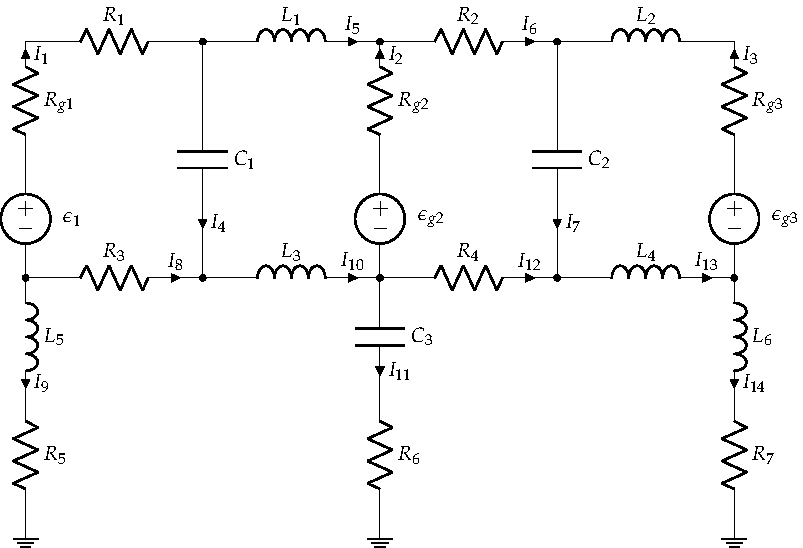
\includegraphics{figuras/mallas_condensadores_bobinas.pdf}
\end{center}


\subsection*{Solución}
Los condensadores se sustituyen por circuitos abiertos (inicialmente
están descargados) y las bobinas por cortocircuitos. De esta forma, el
circuito original queda reducido a tres mallas, como se muestra en la
siguiente figura:

\begin{center}
  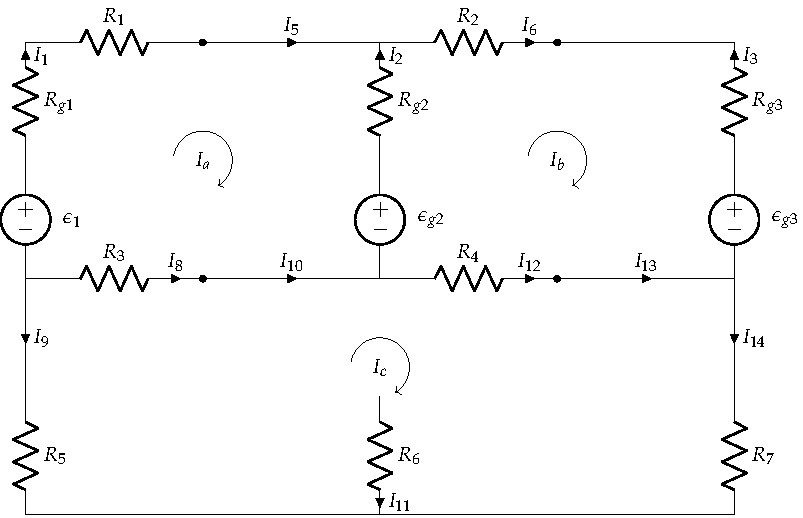
\includegraphics{figuras/mallas_condensadores_bobinas_mod.pdf}
\end{center}


Se resuelve mediante el método de mallas, cuyo sistema de ecuaciones
en forma matricial es:
\begin{equation*}
  \begin{bmatrix}
    12 & -4 & -2 \\
    -4 & 12 & -2\\
    -2 & -2 & 6
  \end{bmatrix}
  \cdot\begin{bmatrix}
         I_a\\
         I_b\\
         I_c
       \end{bmatrix}
       =
       \begin{bmatrix}
         18\\
         2\\
         0
       \end{bmatrix}
     \end{equation*}
     cuya solución es:
     \begin{align*}
       I_{a} & =  \qty{2}{\ampere}\\
       I_{b} & =  \qty{1}{\ampere}\\
       I_{c} & =  \qty{1}{\ampere}
     \end{align*}
     Relacionando estas corrientes de malla con las corrientes de rama
     señaladas en el circuito original (teniendo en cuenta que las
     corrientes que circulan por ramas con condensadores son nulas):
     \begin{align*}
       I_{1} & =  I_{a} = \qty{2}{\ampere}\\
       I_{2} & =  -I_{a}+I_{b} = \qty{-1}{\ampere}\\
       I_{3} & =  -I_{b} = \qty{-1}{\ampere}\\
       I_{4} & =  \qty{0}{\ampere}\\
       I_{5} & =  I_{a} = \qty{2}{\ampere}\\
       I_{6} & =  I_{b} = \qty{1}{\ampere}\\
       I_{7} & =  \qty{0}{\ampere}\\
       I_{8} & =  -I_{a}+I_{c} = \qty{-1}{\ampere}\\
       I_{9} & =  -I_{c} = \qty{-1}{\ampere}\\
       I_{10} & = -I_{a}+I_{c} = \qty{-1}{\ampere}\\
       I_{11} & =  \qty{0}{\ampere}\\
       I_{12} & =  -I_{b}+I_{c} = \qty{0}{\ampere}\\
       I_{13} & =  -I_{b}+I_{c} = \qty{0}{\ampere}\\
       I_{14} & =  I_{c} = \qty{1}{\ampere}
     \end{align*}

     El condensador $C_{1}$ está conectado directamente a la rama
     compuesta por la fuente $E_{2}$ y su resistencia $E_{g2}$ (debido
     a que la bobina se comporta como un cortocircuito). Por tanto,
     suponiendo que la polaridad positiva de este condensador
     corresponde a su borne superior, la tensión de este condensador
     es:
     \begin{equation*}
       U_{C1} = E_{2}-I_{2}\cdot R_{g2} = 22-(-1)\cdot4 = \qty{26}{\volt}
     \end{equation*}
     siendo correcta la polaridad asignada por el signo positivo de
     este resultado. La energía almacenada por el condensador es:
     \begin{equation*}
       E_{C1} = 1/2\cdot V_{C1}^{2}\cdot C_{1} = \qty{0.676}{\milli\joule}
     \end{equation*}

     El condensador $C_{2}$ está conectado directamente a la rama
     compuesta por la fuente $E_{3}$ y su resistencia $E_{g3}$ (debido
     a que la bobina se comporta como un cortocircuito). Por tanto,
     suponiendo que la polaridad positiva de este condensador
     corresponde a su borne superior, la tensión de este condensador
     es:
     \begin{equation*}
       U_{C2} = E_{3}-I_{3}\cdot R_{g3} = 20-(-1)\cdot4 = \qty{24}{\volt}
     \end{equation*}
     siendo correcta la polaridad asignada por el signo positivo de
     este resultado. La energía almacenada por el condensador es:
     \begin{equation*}
       E_{C2} = 1/2\cdot U_{C2}^{2}\cdot C_{2} = \qty{0.576}{\milli\joule}
     \end{equation*}

     El condensador $C_{3}$ está en paralelo con la resistencia
     $R_{4}$ y la resistencia $R_{7}$ (debido a que las bobinas se
     comportan como un cortocircuito y a que por la resistencia
     $R_{6}$ no circula corriente). Por tanto, suponiendo que la
     polaridad positiva de este condensador corresponde a su borne
     superior, la tensión de este condensador es:
     \begin{equation*}
       U_{C3} = I_{12}\cdot R_{4}+I_{14}\cdot R_{7} = 0+1\cdot1 = \qty{1}{\volt}
     \end{equation*}
     siendo correcta la polaridad asignada por el signo positivo de
     este resultado. La energía almacenada por el condensador es:
     \begin{equation*}
       E_{C3} = 1/2\cdot U_{C3}^{2}\cdot C_{3} = \qty{1}{\micro\joule}
     \end{equation*}

     Se calcula ahora el balance de potencias, diferenciando entre
     elementos activos (generadores) y pasivos (receptores):
     \begin{itemize}
     \item Potencia de los generadores:
       \begin{itemize}
       \item $P_{\epsilon1}=\epsilon_1\,I_1=40\cdot 2=\qty{80}{\watt}$
       \item $P_{\epsilon2}=\epsilon_2\,I_2=22\cdot (-1)= \qty{-22}{\watt}$
       \item $P_{\epsilon3}=\epsilon_3\,I_3=20\cdot (-1)= \qty{-20}{\watt}$.
       \end{itemize}
     \item Potencia de las resistencias:
       \begin{itemize}
       \item $P_{Rg1}=R_{g1}\,I_1^2=4\cdot 2^2=\qty{16}{\watt}$
       \item $P_{Rg2}=R_{g2}\,I_2^2=4\cdot (-1)^2=\qty{4}{\watt}$
       \item $P_{Rg3}=R_{g3}\,I_3^2=4\cdot (-1)^2=\qty{4}{\watt}$
       \item $P_{R1}=R_1\,I_1^2=2\cdot 2^2=\qty{8}{\watt}$
       \item $P_{R2}=R_2\,I_6^2=2\cdot 1^2=\qty{2}{\watt}$
       \item $P_{R3}=R_3\,I_8^2=2\cdot (-1)^2=\qty{2}{\watt}$
       \item $P_{R4}=R_4\,I_{12}^2=2\cdot 0^2=\qty{0}{\watt}$
       \item $P_{R5}=R_5\,I_9^2=1\cdot (-1)^2=\qty{1}{\watt}$
       \item $P_{R6}=R_6\,I_{11}^2=1\cdot 0^2=\qty{0}{\watt}$
       \item $P_{R7}=R_7\,I_{14}^2=1\cdot 1^2=\qty{1}{\watt}$
       \end{itemize}
     \end{itemize}
     cumpliéndose que $P_g = P_R = \qty{38}{\watt}$.

%%%%%%%%%%%%%%%%%%%%%%%%%%%%%%%%%%%%%%%%%%%%%%%%%%%%%%%%%%%%%%%%%%
     \section{Enunciado}
     En el circuito de la figura, obtener las intensidades de
     corriente señaladas mediante un análisis por el método de las
     mallas y mediante un análisis por el método de los nudos.

     \vspace{2mm}
     Datos: $\; R_1 = \qty{9}{\ohm}$;\; $R_2 = \qty{4}{\ohm}$;\; $R_3 = \qty{18}{\ohm}$;\; $R_4 = R_5 = R_6 = \qty{20}{\ohm}$;\; $E_1 = \qty{16}{\volt}$;\; $I_g = \qty{2}{\ampere}$

     \begin{center}
       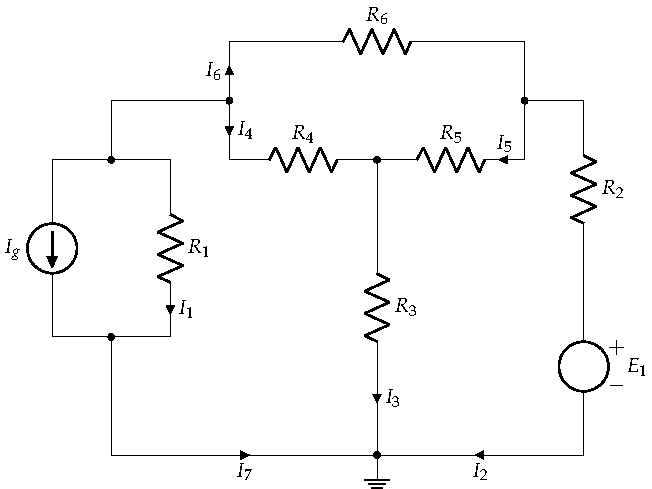
\includegraphics{figuras/BT1_12.pdf}
     \end{center}


     \subsection*{Solución}

     \underline{Resolución mediante mallas}

    \vspace{2mm}
     Se hace la transformación de la fuente de corriente en una fuente
     de tensión:
     \begin{equation*}
       \epsilon_{Ig}=I_g\cdot R_9=2\cdot 9=\qty{18}{\volt}
     \end{equation*}
     Así, el circuito está formado por 3 mallas como se muestra en la
     figura:
     \begin{center}
       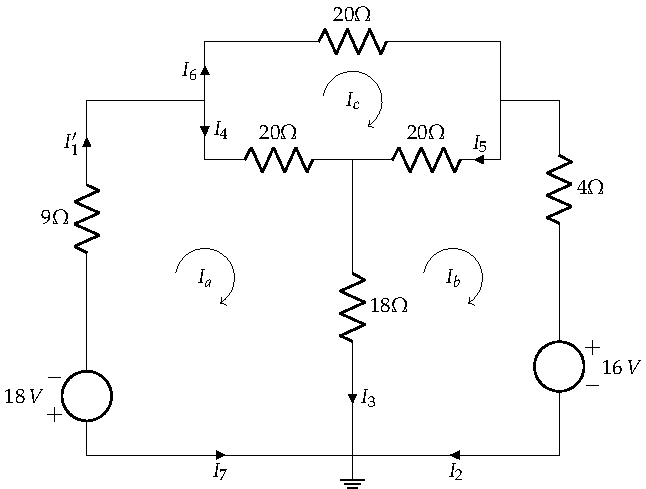
\includegraphics{figuras/BT1_12_mallas.pdf}
     \end{center}
     
     Se plantea el sistema en forma matricial:
     \begin{equation*}
       \begin{bmatrix}
         47 & -18 & -20\\
         -18 & 42 & -20\\
         -20 & -20 & 60
       \end{bmatrix}
       \cdot
       \begin{bmatrix}
         I_a\\
         I_b\\
         I_c
       \end{bmatrix}
       =
       \begin{bmatrix}
         -18\\
         -16\\
         0
       \end{bmatrix}
     \end{equation*}
     cuya solución es:
     \begin{align*}
       I_a&=\qty{-1.26}{\ampere}\\
       I_b&=\qty{-1.33}{\ampere}\\
       I_c&=\qty{-0.87}{\ampere}\\
     \end{align*}
     Estableciendo las relaciones con las corrientes de rama
     indicadas:
     \begin{align*}
       I_1'&=I_a=\qty{-1.26}{\ampere}\\
       I_2&=I_b=\qty{-1.33}{\ampere}\\
       I_3&=I_a-I_b=-1.26-(-1.33)=\qty{0.07}{\ampere}\\
       I_4&=I_a-I_c=-1.26-(-0.87)=\qty{-0.39}{\ampere}\\
       I_5&=I_c-I_b=-0.87-(-1.33)=\qty{0.46}{\ampere}\\
       I_6&=I_c=\qty{-0.87}{\ampere}\\
       I_7&=-I_a=\qty{1.26}{\ampere}\\
     \end{align*}
     La corriente $I_1$ del circuito original se obtiene aplicando el
     1LK:
     \begin{equation*}
       I_g+I_1=I_7\Rightarrow I_1=I_7-I_g=1.26-2=\qty{-0.74}{\ampere}
     \end{equation*}

     \underline{Resolución mediante nudos}

    \vspace{2mm}
     Se transforma la fuente de tensión en una de corriente:
     \begin{equation*}
       I_{\epsilon,g}=\dfrac{\epsilon_g}{R_4}=\dfrac{16}{4}=\qty{4}{\ampere}
     \end{equation*}
     quedando el circuito que se muestra en la figura:
     \begin{center}
       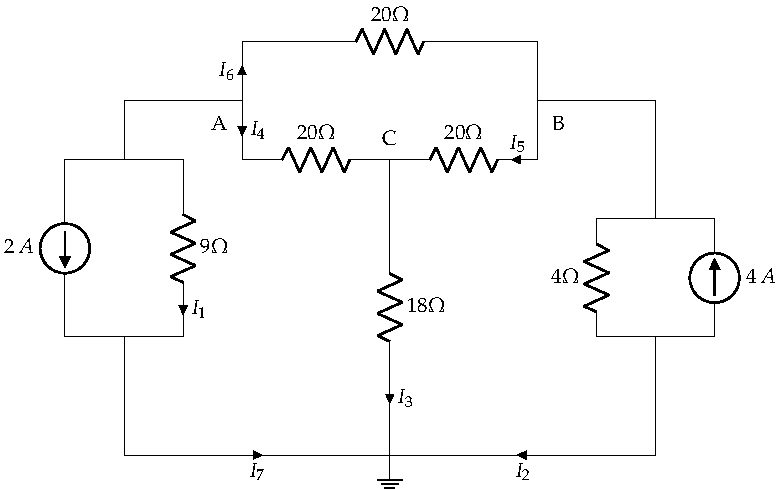
\includegraphics{figuras/BT1_12_nudos.pdf}
     \end{center}
     Con los nudos indicados, se aplica el método de nudos en su forma
     matricial:
     \begin{equation*}
       \begin{bmatrix}
         \dfrac{19}{90} & -\dfrac{1}{20} & -\dfrac{1}{20}\\[10pt]
         -\dfrac{1}{20} & \dfrac{7}{20} & -\dfrac{1}{20}\\[10pt]
         -\dfrac{1}{20} & -\dfrac{1}{20} & \dfrac{7}{45}
       \end{bmatrix}
       \cdot
       \begin{bmatrix}
         U_A\\
         U_B\\
         U_C
       \end{bmatrix}
       =
       \begin{bmatrix}
         -2\\
         4\\
         0
       \end{bmatrix}
     \end{equation*}
     cuya solución es:
     \begin{align*}
       U_A&=\qty{-6.64}{\volt}\\
       U_B&=\qty{10.66}{\volt}\\
       U_C&=\qty{1.29}{\volt}\\
     \end{align*}
     A partir de 1LK, 2LK y ley de Ohm, se obtienen las corrientes
     indicadas:
     \begin{align*}
       I_1&=\dfrac{U_A}{R_9}=\dfrac{-6.64}{9}=\qty{-0.74}{\ampere}\\[7pt]
       I_2&= I_{R_4}-I_{\epsilon,g}=\dfrac{U_B}{R_4}-4=\dfrac{10.66}{4}-4=\qty{-1.34}{\ampere}\\[7pt]
       I_3&=\dfrac{U_C}{R_{18}}=\dfrac{1.29}{18}=\qty{0.07}{\ampere}\\[7pt]
       I_4&=\dfrac{U_{AC}}{R_{20}}=\dfrac{U_A-U_C}{R_{20}}=\dfrac{-6.64-1.29}{20}=\qty{-0.39}{\ampere}\\[7pt]
       I_5&=\dfrac{U_{BC}}{R_{20}}=\dfrac{U_B-U_C}{R_{20}}=\dfrac{10.66-1.29}{20}=\qty{0.47}{\ampere}\\[7pt]
       I_6&=\dfrac{U_{AB}}{R_{20}}=\dfrac{U_A-U_B}{R_{20}}=\dfrac{-6.64-10.66}{20}=\qty{-0.87}{\ampere}\\[7pt]
       I_7&=I_g+I_1
     \end{align*}

     Se observa que los valores obtenidos son idénticos con ambos
     métodos.

    \section{Enunciado}

    Resolver el circuito por el método que se estime conveniente, obteniendo:
    \begin{itemize}
        \item El valor de las corrientes indicadas ($I_1, I_2, I_3, I_4, I_5$).
        
        \item La carga y polaridad de $C_1, C_2$ y $C_3$.

        \item La potencia entregada o absorbida por los elementos activos.
    \end{itemize}
    
    \begin{minipage}{0.65\linewidth}
      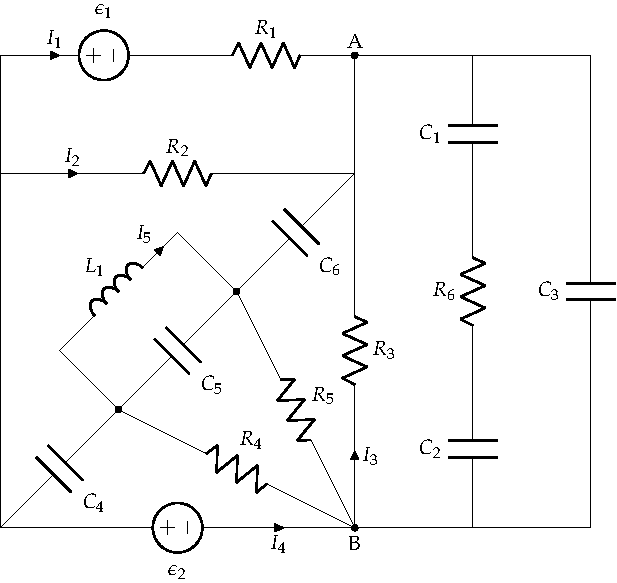
\includegraphics[scale=0.9]{figuras/BT1_ej14_enunciado.pdf}
    \end{minipage}
    \begin{minipage}{0.35\linewidth}
    
        \hspace{5mm}Datos:
    
        \vspace{2mm}    
        \hspace{5mm}$R_1 = R_2 = \qty{2}{\ohm}$
    
        \vspace{1mm}
        \hspace{5mm}$R_3 = R_4 = R_5 = R_6 = \qty{1}{\ohm}$
    
        \vspace{1mm}
        \hspace{5mm}$C_i = i\,\si{\micro\farad}$
    
        \vspace{1mm}
        \hspace{5mm}$L_1 = 1\,\si{\milli\henry}$
    
        \vspace{1mm}
        \hspace{5mm}$\epsilon_1 = \qty{10}{\volt}$
    
        \vspace{1mm}
        \hspace{5mm}$\epsilon_2 = \qty{10}{\volt}$
        
    \end{minipage}

    \subsection*{Solución}
    Para analizar el circuito, sustituimos los condensadores por circuito abierto, y la bobina por cortocircuito:

    \vspace{2mm}
    \begin{minipage}{0.3\linewidth}
      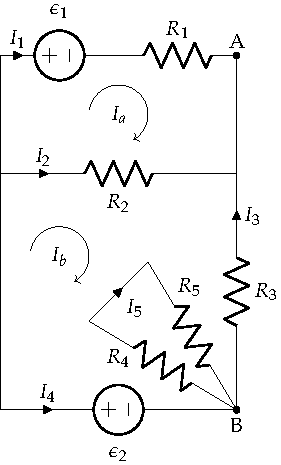
\includegraphics[scale=0.98]{figuras/BT1_ej14_mallas.pdf}
    \end{minipage}
    \hfill
    \begin{minipage}{0.65\linewidth}
    
        \vspace{-5mm}
        En el circuito resultante: $I_5=0$, $I_3=I_4$.
    
        \vspace{3mm}
        Resolviendo por mallas, definiendo las corrientes de malla $I_a$ e $I_b$ en sentido horario:
    
        %\vspace{3mm}
        \begin{minipage}{0.53\linewidth}
          \begin{equation*}
            \begin{bmatrix}
                R_1+R_2 & -R_2 \\[4pt]
                -R_2 & R_2+R_3
            \end{bmatrix} \cdot %
            \begin{bmatrix}
                I_a\\[4pt]
                I_b
            \end{bmatrix} = %
            \begin{bmatrix}
                -\epsilon_1\\[4pt]
                \epsilon_2
            \end{bmatrix}
        \end{equation*}
        \end{minipage}
        \hfill
        \begin{minipage}[c]{0.02\linewidth}
            \vspace{3mm}
            $\xrightarrow{\hspace*{0.2cm}}$ % https://latex.org/forum/viewtopic.php?t=3894
        \end{minipage}
        \hfill
        \begin{minipage}{0.4\linewidth}
            \begin{equation*}
                \begin{bmatrix}
                    4 & -2 \\[4pt]
                    -2 & 3
                \end{bmatrix} \cdot %
                \begin{bmatrix}
                    I_a\\[4pt]
                    I_b
                \end{bmatrix} = %
                \begin{bmatrix}
                    -10\\[4pt]
                    10
                \end{bmatrix}
            \end{equation*}
        \end{minipage}
    
        \vspace{3mm}
        \[
            I_a = \qty{-1.25}{\ampere} \; , \qquad I_b = \qty{2.5}{\ampere}
        \]
    
        \vspace{2mm}
        \hspace{3mm}Luego las corrientes de rama pedidas son:
    
        \vspace{-1mm}
        \[
            I_1 = I_a = \boxed{\qty{-1.25}{\ampere}} \; , \quad 
            I_2 = I_b - I_a = \boxed{\qty{3.75}{\ampere}} \; ,
        \]
        \[
            I_3 = I_4 = -I_b = \boxed{\qty{-2.5}{\ampere}} \; , \quad
                \boxed{I_5 = \qty{0}{\ampere}}
        \]
    \end{minipage}
    
    \vspace{2mm}
    
    Si no se hubiera visto inmediatamente que $I_5=0$, siempre podría haberse definido una tercera corriente de malla, $I_c=I_5$, con lo que el sistema de ecs. quedaría:
    \begin{equation*}
        \begin{bmatrix}
            R_1+R_2 & -R_2 & 0\\[4pt]
            -R_2 & R_2+R_3 & 0\\[4pt]
            0 & 0 & R_4+R_5
        \end{bmatrix} \cdot %
        \begin{bmatrix}
            I_a\\[4pt]
            I_b\\[4pt]
            I_c
        \end{bmatrix} = %
        \begin{bmatrix}
            -\epsilon_1\\[4pt]
            \epsilon_2\\[4pt]
            0
        \end{bmatrix}
    \end{equation*}
    La tercera ecuación no tiene incógnitas en común con las dos primeras, y de ella se obtiene directamente $I_c=I_5=0$.
    
    \vspace{4mm}
    Para calcular la carga en los condensadores, hay que tener en cuenta que, al no circular corriente por $R_6$ en régimen permanente del circuito, su tensión es de \qty{0}{\volt}. Luego la asociación serie de $C_1$ y $C_2$ está sometida a la tensión $U_{AB}$.
    
    \vspace{2mm}
    Asumiendo polaridad positiva en el punto A, la carga de $C_3$ es: 
    \[ 
        q_3 = C_3 \cdot U_{C_3} = C_3 \cdot (-I_3 \cdot R_3) = \boxed{\qty{7.5}{\micro\coulomb}} 
    \]
    
    \vspace{2mm}
    La carga de la asociación serie de $C_1$ y $C_2$, asumiendo polaridad positiva en A, es:
    \[ 
        q_{\textrm{serie}} = C_{12} \cdot U_{C_{12}} = C_{12} \cdot (-I_3 \cdot R_3) = \dfrac{5}{3}\,\si{\micro\coulomb} 
    \]
    
    donde la capacidad equivalente de la asociación serie ha sido calculada como: 
    \[ 
        C_{12} = \dfrac{C_1 \cdot C_2}{C_1 + C_2} = \dfrac{2}{3}\,\si{\micro\farad} 
    \]

    \vspace{-2mm}
    Al estar $C_1$ y $C_2$ asociados en serie, su carga es la misma, luego \( q_{\textrm{serie}} = \boxed{q_1 = q_2 = \dfrac{5}{3}\,\si{\micro\coulomb}} \)
    
    \vspace{3mm}
    Finalmente, la potencia entregada por los elementos activos es:
    \[ 
        P_{\epsilon1} = \epsilon_1 \cdot (-I_1) = \boxed{\qty{12.5}{\watt}}
        \qquad \qquad 
        P_{\epsilon2} = \epsilon_2 \cdot (-I_4) = \boxed{\qty{25}{\watt}} 
    \]
    

%%% Local Variables:
%%% mode: latex
%%% TeX-master: "Problemas_TC"
%%% ispell-local-dictionary: "castellano"
%%% End:

